\documentclass[11pt, oneside]{article}   	% use "amsart" instead of "article" for AMSLaTeX format
\usepackage{geometry}                		% See geometry.pdf to learn the layout options. There are lots.
\geometry{a4paper}                   		% ... or a4paper or a5paper or ... 
%\geometry{landscape}                		% Activate for rotated page geometry
%\usepackage[parfill]{parskip}    		% Activate to begin paragraphs with an empty line rather than an indent
\usepackage{graphicx}				% Use pdf, png, jpg, or eps§ with pdflatex; use eps in DVI mode
								% TeX will automatically convert eps --> pdf in pdflatex		
\usepackage{amssymb}
\usepackage{amsmath}
\usepackage{authblk}
\usepackage{graphicx}

\usepackage{url}

%SetFonts

%SetFonts
\title{A Global Digital Assurance Framework for Integrating Essential Ecosystem Features within a Stable, Diverse and Extensive Alarm Management Platform}
\author{Dr Aidan Thomas Parkinson\\ Realfeed Ltd., Sinsuran, West End, Wedmore, Somerset, BS28 4BW.\\ aidan.parkinson@gmail.com}
\date{\today}							% Activate to display a given date or no date

\begin{document}
\maketitle

\section*{Abstract}

\pagebreak

\section{Introduction}
Digital platform governance involves thoughtful considerations towards the standardisation of interfaces to enable a diverse market of complementors to find opportunity in developing services for consumers.
There has been much discussion about the creation of platforms that seek network effects to deliver a popular market share of consumers with compelling development opportunities for complimentors to offer proprietary tools to enhance personal utility.
Such an approach has been very successful for exploiting new domains, such as the internet and personal devices.
However, such contributions may be somewhat detremental in addressing societies pressing contractual problems involved in minimum security standards to govern a limited natural ecosystem.
Loss of biodiversity, frameworks to limit global temperature rise, social unrest and military intervention are all relevant demonstrations in this domain and appear to exhbit some common features.\

One potential area of conflict in ecosystem governance is the management of competing principles of what is Good.
This involves a definition that not only justifies ecosystem ethical priorities, but also a recognition of what is Sovereign.
Minimal policies could then be identified to contribute towards ecosystem stability and align supply-chains with a natural course of development.\

Another important aspect is the identification of Frameworks and Guidance that signal the failure of Features to successfully integrate with an ecosystem.
Failure is an important feedback mechanism for developers to learn and adapt work-in-progress Features and, hence, enforcement need ideally to be rapid, consistent and relevant.
It has been recognised that practical networking of outstations and sensors in the field with public domains has historically been poorly enforced.
Lack of consumer confidence has contributed to sluggish market penetration of internet-of-things technologies to-date.\

Further, it appears important to consider the management of Intellectual Property and how governing agents may operate.
Such thought needs to reflect on the ecosystems ethical priorities, competition and operational costs.\

Therefore, this article asks the question: \emph{"How could one govern an alarm management platform to support a stable and diverse natural ecosystem?"}
The discussion draws upon experience of practice and a wide-ranging review of theory.
In conclusion an Ontology that offers a personal perspective on this question is proposed.
It is acknowledged that the problems faced are formidable and no solution can be perfect.
However, it is intended that this article contributes common-sense that may inspire the sustainable development of new technologies going forward.\


\section{Ethics}
It is acknowledged that any ecosystem may include agents with different interests and potentially competing principles of what is Good.
However, it is extremely challenging to identify a global perspective of what a Good interest is.
In an attempt to govern a natural ecosystem, one could understand that a process of identification involves considering prevailing representations of the State of Nature.
Two influential and conflicting accounts of the State of Nature are found in John Locke [?????] and Thomas Hobbes' Leviathan.\

Thomas Hobbes... [to be summarised]...
Through taking the Hobbesian perspective into account, we may be led to the contributions of John Rawls as a substantive governance system for managing competing principles of the good.\

John Locke... [to be summarised]...
Following John Locke one could arrive at Robert Nozick's challenge to the Rawlsian view... [to be summarised].\

Ultimately, it appears that the perspective of Locke is undermined by the practical facts that there is no way of assuring an initial state of Utopia and that natural disasters cannot be bargained with.
Therefore, it is the Rawlsian view that influence an Executive Function here. An account of which follows.\

\subsection{Minimum Decency}

Rawls'~\cite{jr1} full statement of justice for institutions is a concise and widely recognised solution to the priority problem of justice as fairness. A sense of which I wish to share and apply. An account, but not a defence, follows.

\subsubsection{First principle}

\begin{quote}
"Each person is to have an equal right to the most extensive total system of equal basic liberties compatible with a similar system of liberty for all."
\end{quote}

\subsubsection{Second principle}

\begin{quote}
"Social and economic inequalities are to be arranged so that they are both:
\begin{description}
\item[ a)] to the greatest benefit of the least advantaged, consistent with the just savings principle, and
\item[ b)] attached to offices and positions open to all under conditions of fair equality of opportunity."
\end{description}
\end{quote}

\subsubsection{First priority rule: the priority of liberty}

\begin{quote}
"The principles of justice are to be ranked in lexical order and therefore liberty can be restricted only for the sake of liberty.
There are two cases:
\begin{description}
\item[ a)] a less extensive liberty must strengthen the total system of liberty shared by all;
\item[ b)] a less than equal liberty must be acceptable to those with lesser liberty."
\end{description}
\end{quote}

\subsubsection{Second priority rule: the priority of justice over efficiency and welfare}

\begin{quote}
"The second principle of justice is lexically prior to the principle of efficiency and to that of maximising the sum of advantages; and fair opportunity is prior to the difference principle. There are two cases:
\begin{description}
\item[ a)] an inequality of opportunity must enhance the opportunities of those with the lesser opportunity;
\item[ b)] an excessive rate of saving must on balance mitigate the burden of those bearing the hardship."
\end{description}
\end{quote}

\subsubsection{General conception}

\begin{quote}
"All social primary goods---liberty and opportunity, income and wealth, and the bases of self-respect---are to be distributed equally unless an unequal distribution of any or all of these goods is to the advantage of the least favoured."
\end{quote}

\subsection{Rate of saving}

Rawls' second priority rule stipulates a requirement to control rates of saving, so that excessive rates on balance mitigate the burden of those bearing the hardship. Therefore, there is a requirement to estimate the present generations rate of saving. This returns an aggregation of the well-being of individuals, often described as \emph{intergenerational well-being}.

\subsubsection{Cost-benefit analysis}

Dasgupta~\cite{pd2} explains how we \emph{value} when comparing objects and we \emph{evaluate} when comparing the benefits of actions. Valuation and evaluation both involve comparisons between worlds with and without the course of action or object. This process is called social cost-benefit analysis and involves measuring consumer and producer \emph{surpluses}. Carrying out social cost-benefit analysis requires a quantitative formulation of intergenerational well-being, for which Ramsey's Mathematical Theory of Saving~\cite{fr1} is a well respected candidate and can be summarised as follows:

\begin{equation}
V_t = \sum_t^\infty \beta^{(\tau - t)} \cdot U (C_\tau)
\qquad \text{for }
\qquad t \geq 0
\end{equation}

where,
\begin{equation}
\beta = \frac{1}{(1+\mu)}
\end{equation}

Where, $V_t$ is \emph{intergenerational well-being}, $\beta$ is the \emph{discount factor}, $U$ is \emph{well-being}, $C_\tau$ is \emph{consumption during time-step}, $t$ is \emph{time} and $\mu$ the \emph{social discount-rate}.

\begin{equation}
\mu = \sigma \cdot g + \delta
\end{equation}

Where, $\sigma$ is the \emph{marginal utility of consumption} and the difference in the utility one would gain from a unit of consumption by those of low and high incomes, $g$ is the \emph{long- term growth rate} in consumption, $\delta$ is the \emph{pure rate of time preference} and our impatience to consume resources in fear of extinction.

\begin{equation}
S = \frac{\mu-\delta}{\sigma \cdot \mu}
\end{equation}

Where, $S$ is the \emph{savings rate} and the proportion of output that should be invested.

In practical applications, $U (C_\tau)$ can be substituted for net cash-flow in time period to yield a familiar equation.

\subsubsection{Accounting}

To establish estimates for rates of saving it is necessary to account for circumstances with and without a course of action or object. There are a broad range of influences on well-being that need to be accounted for. Here an original convenient taxonomy is proposed in illustrated in Figure~\ref{Influences on well-being figure}, inspired somewhat by Dasgupta~\cite{pd3}.

\begin{figure}[h]
\begin{center}
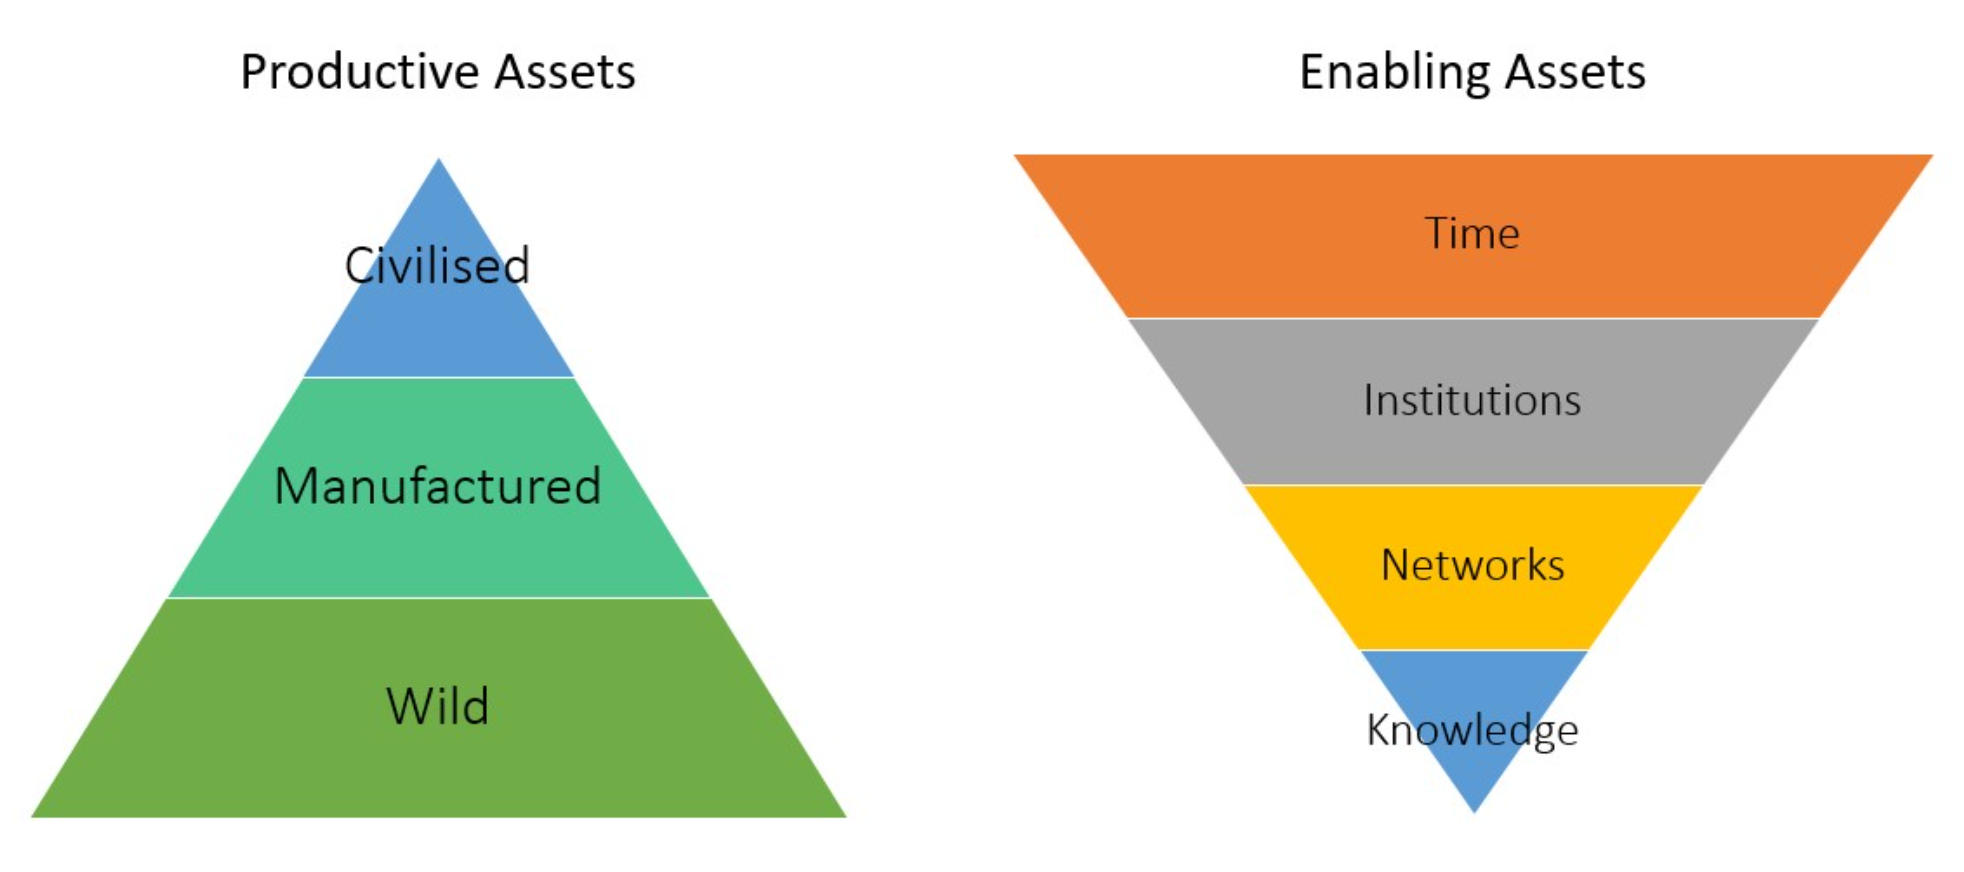
\includegraphics[width=0.75\textwidth]{productiveAssetTaxonomy.png}
\caption{Original taxonomy of influences on human well-being}
\label{Influences on well-being figure}
\end{center}
\end{figure}

Enabling assets allow society to be more precise about their influences on the physical environment, may be defined as software and possibly released for mass production. Dasgupta\cite{pd2} also describes how enabling and production assets can exhibit different types of value:

\begin{description}
\item[Use-value:] the contribution of an asset to well-being once consumed;
\item[Intrinsic-value:] the contribution of an asset to well-being in the understanding that it exists (e.g. believing that polar bears roam free in the arctic);
\item[Option-value:] the contribution of an asset to well-being in the understanding that it may be consumed at some point in the future.
\end{description}

The attitudes and preferences that characterise a state of well-being are not defined and need to be found. Recognised methods to evaluate social attitudes and preferences are:

\begin{description}
\item[Stock markets:] Determines the values of a supply of commodities through a process of market clearing.
\item[Hedonic regression:] Determines the value of amenities by comparing house prices and the amenities available on different parcels of land to each other using regression analysis.
\item[Satisfaction/approval surveys:] Determines the level of approval from a representative sample of respondents for a particular amenity. Arrow et al.~\cite{kja1} recognised that respondent heuristics prevent valuation of an amenity using survey methods.
\end{description}

\subsubsection{Limitations}

Often, one's own activities can yield personal benefits at the expense of those who have no interest.
Environmental pollution is a good example, where the impacts upon others may not be accounted for by the source.
Coase~\cite{rc1} has demonstrated that by collecting reliable information about the precise sources of these activities and impacts on property rights effective resolutions can be found.\
\emph(Wild Capital), by its very nature, does not submit to any social contract governing the state (A pre-requisite for currency).
Therfore, no human can confidently place a valuation on Wild Capital and it's contributions to well-being may be priceless.\
Cost-benefit analysis involves a number of personal assumptions that may not be particularly relevant to many people. This tool for decision-making is best suited to personal savings behaviour.
Cost-benefit analysis may be entirely inappropriate for decisions relating to \emph(essential goods).
Attention to distribution outliers and qualitative information is essential in assuring a just approach to personal savings goals.

\subsubsection{A Note on Perfectionism}

There is a body of thought that define the duty and obligations of individuals so as to maximise the achievement of human excellence in art, science and culture. Neitzsche~\cite{gam1} states:
\begin{quote}
"Mankind must work continually to produce individual great human beings---this and nothing else is the task... for the question is this: how can your life, the individual life, retain the highest value, the deepest signfiicance?... Only by your living for the good of the rarest and most valuable specimens."
\end{quote}
However, in order to arrive at perfectionism, Rawls~\cite{jr2} asserts that we would have to attribute all parties to a prior acceptance of a certain style and aesthetic grace, and to advance the the pursuit of knowledge and the cultivation of the arts. Whilst I believe values of excellence may be recognised, human principles need to be pursued within the limits of the principle of free association. The coercive apparatus of the state would not be used to win greater liberty or larger shares of wealth on the grounds that ones activities are of more intrinsic value. The social resources necessary to support associations dedicated to advancing the arts, sciences and culture generally are to be won as a fair return for services rendered, or from such voluntary contributions as citizens wish to make. The state might limit its support to cases of overcoming isolation and assurance.



\section{Failure}


\section{Operations}


\section{Conclusions}

\begin{thebibliography}{99}

\bibitem{kja1} Arrow~K.J. Solow~R.M. Portney~P. Leamer~E. Radner~R.; Schuman~H. (1993)
\emph{Report of NOAA Panel on Contingent Valuation.},
Federal Register, pp. 4601-46014
	
\bibitem{rc1} Coase~R.H. (1960)
\emph{The Problem of Social Cost.},
The Journal of Law and Economics, 3, pp. 1-44
	
\bibitem{pd2} Dasgupta~P. (2001)
\emph{Valuing Goods.},
In: Human Well-Being and the Natural Environment. Oxford: Oxford University Press, pp. 122-138
	
\bibitem{pd3} Dasgupta~P. (2015)
\emph{Disregarded Capitals: What National Accounting Ignores.},
Accounting and Business Research, 45(4), pp. 122-138
	
\bibitem{gam1} Morgan~G.A. (1941)
\emph{What Nietzsche Means.}
Cambridge, MA: Harvard University Press
	
\bibitem{fr1} Ramsey~F.P. (1928)
\emph{A Mathematical Theory of Saving.}
Economic Journal, 38(152) pp. 543-559
	
\bibitem{jr1} Rawls~J. (1971)
\emph{Further Cases of Priority.}
In: A Theory of Justice. Cambridge, MA and London: Harvard University Press, pp. 298-303
	
\bibitem{jr2} Rawls~J. (1971)
\emph{The Principle of Perfection.}
In: A Theory of Justice. Cambridge, MA and London: Harvard University Press, pp. 325-332

\end{thebibliography}

\end{document}  
